\chapter{Cotas superiores mínimas}

%------------------- Definición 8.1
\begin{tcolorbox}
    \begin{def.}
	Un conjunto $A$ de números reales está acotado superiormente si existe un número $x$ tal que 
	\begin{center}
	    $x\geq a$ para todo $a$ de $A$.
	\end{center}
	este número $x$ se denomina una cota superior de $A$.\\\\
    $A$ está acotado superiormente si y sólo si existe un número $x$ que es una cota superior de $A$.(y en este caso existirán muchas cotas superiores de $A$);\\\\
    \end{def.}
\end{tcolorbox}

%------------------- Definición 8.2
\begin{tcolorbox}
    \begin{def.}
	Un número $x$ es una cota superior mínima de $A$ si
	\begin{enumerate}[\bfseries (1)]
	    \item $x$ es una cota superior de $A$,
	    \item si $y$ es una cota superior de $A$, entonces $x\leq y$.
	\end{enumerate}
	El término \textbf{supremo} de $A$ es sinónimo al de cota superior mínima y tiene una ventaja: se puede abreviar mediante un símbolo muy adecuado
	$$\sup A$$
    \end{def.}
\end{tcolorbox}
\vspace{0.2cm}

    Si $x$ e $y$ son ambos cotas superiores mínimas de $A$, entonces $x=y$.\\\\
	Demostración.-\; En efecto, en este caso
	\begin{center}
	\begin{tabular}{ll}
	    $x\leq y,$ & ya que $y$ es una cota superior, y $x$ es una cota superior mínima,\\
	    $y\leq x$ & ya que $x$ es un cota superior, e $y$ es una cota superior mínima.
	\end{tabular}
	\end{center}
	por lo tanto, $x=y$. \\\\

%------------------- Definición 8.3
\begin{tcolorbox}
    \begin{def.}
	Un conjunto $A$ de números reales está acotado inferiormente si existe un número $x$ tal que
	\begin{center}
	    $x\leq a$ para todo $a$ de $A$.
	\end{center}
	Dicho número $x$ se denomina una cota inferior de $A$.
    \end{def.}
\end{tcolorbox}

\begin{tcolorbox}
    \begin{def.}
	Un número $x$ es la cota inferior máxima de $A$ si
	\begin{enumerate}[\bfseries (1)]
	    \item $x$ es una cota inferior de $A$, y
	    \item si $y$ es una cota inferior de $A$, entonces $x\geq y$.
	\end{enumerate}
	La cota inferior máxima de $A$ se denomina también el \textbf{ínfimo} de $A$, abreviadamente
	$$\inf A$$
    \end{def.}
\end{tcolorbox}

%------------------- P13
\begin{tcolorbox}
\begin{prop}[Propiedad de la cota superior mínima]
    Si $A$ es un conjunto de números reales, $A\neq \emptyset$, y $A$ está acotado superiormente, entonces $A$ posee una cota superior mínima. 
\end{prop}
\end{tcolorbox}

El enorme significado de P13 se hará patente sólo de manera gradual, aunque ya estamos en condiciones de comprobar su importancia dando las demostraciones que omitimos en el Capítulo 7.\\


\setcounter{chapter}{7}
\setcounter{teo}{0}
\begin{teo}
    Si $f$ es continua en $[a,b]$ y $f(a)<0<f(b)$, entonces existe algún número $x$ de $[a,b]$ tal que $f(x)=0.$\\\\
	Demostración.-\; La demostración es tan sólo una versión rigurosa del método esbozado al final del capítulo 7: localizaremos el menor número $x$ de $[a,b]$ tal que $f(x)=0$.\\
	Definamos el conjunto $A$, de la manera siguiente:

	$$A=\lbrace x:a\leq x \leq b, \; \mbox{y}\; f \; \mbox{negativa en en el intervalo}\; [a,x]\rbrace.$$

	Obviamente $A\neq \emptyset$ ya que $a$ pertenece a $A$; de hecho, existe un $\delta >0$  tal que $A$ contiene a todos los puntos $x$ que satisfacen $a\leq x < a+\delta$ ya que $f$ es continua en $[a,b]$ y $f(a)<0$. Análogamente, $b$ es una cota superior de $A$ y, de hecho, existe un $\delta>0$ tal que todos los puntos $x$ que satisfacen $b-\delta<x\leq b$ son cotas superiores de $A$; esto también se deduce del Problema 6-16, ya que $f(b)>0$.\\
	A partir de estas observaciones se deduce que $A$ posee cota superior mínima $\alpha$ y que $a<\alpha<b$. Ahora demostraremos que $f(\alpha)=0$, excluyendo las posibilidades $f(\alpha)<0$ y $f(\alpha)>0$.\\
	Supongamos primero que $f(\alpha)<0$. Según el teorema 6-3, existe un $\delta>0$ tal que $f(x)<0$ si $\alpha- \delta<x<\alpha+\delta$. Ha de existir un número $x_0$ de $A$ que satisface $\alpha-\delta<x_0<\alpha$ (ya que sino $\alpha$ no sería la mínima cota superior de $A$). Esto significa que $f$ es negativa en todo el intervalo $[a,x_0]$. Pero si $x_1$ es un número situado entre $\alpha$ y $\alpha+\delta$, entonces $f$ también es negativa en todo el intervalo a $A$. Pero esto contradice el hecho de que $\alpha$ sea una cota superior de $A$; concluimos pues que la suposición que hemos hecho anteriormente, de que $f(\alpha)<0$ sebe ser falsa.\\
	Supongamos ahora que $f(\alpha)>0$. Entonces existe un número $\delta>0$ tal que $f(x)>0$ si $\alpha-\delta<x<\alpha+\delta$. Una vez más, sabemos que existe un $x_0$ de $A$ que satisface $\alpha-\delta<x_0<\alpha$; pero esto significa que $f$ es negativa en $[a,x_0]$, lo cual es imposible ya que $f(x_0)>0$. Así pues, la suposición de que $f(\alpha)>0$ conduce a una contradicción, quedando sólo la posibilidad de que $f(\alpha)=0$.\\
\end{teo}

Las demostraciones de los teoremas 2 y 3 del capítulo 7 requieren un sencillo resultado preliminar, que va a desempeñar una función muy similar a la del teorema 6-3 en la demostración anterior.\\\\

\setcounter{chapter}{8}
\setcounter{teo}{0}

\begin{teo}
    Si $f$ es continua en $a$, existe un número $\delta>0$ tal que $f$ está acotada superiormente en el intervalo $(a-\delta,a+\delta)$.\\\\
    Demostración.-\; Como el $\lim\limits_{x\to a} f(x) =f(a)$, para cada $\epsilon>0$, existe un $\delta>0$ tal que, para todo $x$,
    \begin{center}
	si $|x-a|<\delta$, entonces $|f(x)-f(a)|<\epsilon,$
    \end{center}
    Tan sólo es necesario aplicar esta propiedad a algún $\epsilon$ en particular, por ejemplo $\epsilon=1$. Deducimos pues que existe un $\delta>0$ tal que, para todo $x$,

    \begin{center}
	si $|x-a|<\delta$, entonces $|f(x)-f(a)|<1,$
    \end{center}

    y, en particular, si $|x-a|<\delta$ entonces $f(x)-f(a)<1$. Esto completa la demostración: en el intervalo $(a-\delta,a+\delta)$ la función $f$ está acotada superiormente por $f(a)+1.$\\\\
\end{teo}

Por supuesto, ahora podríamos demostrar también que $f$ está acotada inferiormente en algún intervalo $(a-\delta,a+\delta)$, concluyendo, por tanto, que $f$ está acotada en algún intervalo abierto que contiene a $a$.\\
En este sentido, cabe destacar en particular la observación de que si $\lim\limits_{x\to a^{+}},$ entonces existe un $\delta>0$ tal que $f$ está acotada en el conjunto $\lbrace x:a\leq x < a+\delta\rbrace$, pudiendo hacerse una observación análoga si $\lim\limits_{x\to b^-}=f(b)$.\\\\

\setcounter{chapter}{7}
\setcounter{teo}{1}
\begin{teo}
    Si $f$ es continua en $[a,b]$, entonces $f$ está acotada superiormente en $[a,b]$.\\\\
	Demostración.-\; Sea,
	$$A=\lbrace x:a\leq x \leq b \;\mbox{y}\; f \; \mbox{está acotada superiormente en}\; [a,x]\rbrace$$
	Obviamente $A\neq \emptyset$ (ya que $a$ pertenece a $A$), y está acotada superiormente por $b$, de manera que $A$ posee una cota superior mínima $\alpha$. Observemos que estamos aplicando el término acotado superiormente tanto al conjunto $A$, localizado en el eje horizontal, como a la función $f$, es decir, a conjuntos del tipo $\lbrace f(y):a\leq y \leq x\rbrace$, localizados en el eje vertical.\\
	La primera etapa de la demostración consiste en probar que $\alpha=b$. Supongamos, por el contrario, que $a<b$. Según el teorema 1 existe un $\delta >0$ tal que $f$ está acotada en $(a-\delta,a+\delta)$. Como $\alpha$ es la cota superior mínima de $A$ existe algún $x_0$ de $A$ que satisface $\alpha-\delta<x_0<\alpha$. Esto significa que $f$ está acotada en $[a,x_0]$. Pero si $x_1$ es cualquier número tal que $\alpha<x_1<\alpha+\delta$, entonces $f$ también está acotada en $[x_0,x_1]$. Por lo tanto $f$ está acotada en $[a,x_1]$, de manera que $x_1$ pertenece a $A$, lo que contradice el hecho de que $\alpha$ sea una cota superior a $A$. Esta contradicción demuestra que $\alpha=b$. Debemos mencionar un detalle: en la demostración hemos puesto implícitamente que $a<\alpha$ de manera que $f$ está definida en algún intervalo $(\alpha-\delta,\alpha+\delta)$; la posibilidad $a=\alpha$ puede excluirse de manera similar, utilizando el hecho de que existe un $\delta>0$ tal que $f$ está acotada en $\lbrace x:a\leq x < a + \delta\rbrace$.\\
	La demostración todavía no es completa; únicamente sabemos que $f$ está acotada en $[a,x]$ para todo $x<b$, no necesariamente que $f$ está acotada en $[a,b]$. Sin embargo, sólo es necesario añadir una pequeña observación.\\
	Existe un $\delta>0$ tal que $f$ está acotada en $\lbrace x:b-\delta < x \leq b \rbrace$. Existe también un $x_0$ de $A$ tal que $b-\delta<x_0<b$. De manera que $f$ está acotada en $[a,x_0]$ y también en $[x_0,b],$ por tanto $f$ está acotada en $[a,b]$.\\\\
\end{teo}

%-------------------- teorema 7.3
\begin{teo}
    Si $f$ es continua en $[a,b]$, entonces existe un número $y$ de $[a,b]$ tal que $f(y)\geq f(x)$ para todo $x$ de $[a,b]$.\\\\
	Demostración.-\; Sabemos que $f$ está acotada en $[a,b]$, lo que significa que le conjunto
	$$\lbrace f(x):x \mbox{ pertenezca a }[a,b]\rbrace$$
	está acotado. Además, dicho conjunto es, obviamente, distinto del $\emptyset$, de manera que admite una cota superior mínima $\alpha$. Como $\alpha\geq f(x)$ para $x$ de $[a,b]$, basta demostrar que $\alpha=f(y)$ para algún $y$ de $[a,b]$.\\
	Supongamos, por el contrario, que $\alpha\neq f(y)$ para todo $y$ de $[a,b]$. Entonces la función $g$ definida mediante
	$$g(x)=\dfrac{1}{\alpha-f(x)},\quad x\in [a,b]$$
	es continua en $[a,b]$, ya que el denominador de la expresión del lado derecho de la igualdad nunca vale $0$. Por otra parte, $\alpha$ es la mínima cota superior de $\lbrace f(x):x \mbox{ pertenezca a }[a,b] \rbrace$, esto significa que 
	\begin{center}
	    para cada $\epsilon > 0$ existe un $x$ de $[a,b]$ con $\alpha - f(x)<\epsilon$.
	\end{center}
	Esto, a su vez, significa que 
	\begin{center}
	    para cada $\epsilon > 0$ existe un $x$ de $[a,b]$ con $g(x)>1/\epsilon$.
	\end{center}
	Pero esto quiere decir que $g$ no está acotada en $[a,b]$, lo que contradice el resultado del teorema anterior.\\\\
\end{teo}

\setcounter{chapter}{8}
\setcounter{teo}{1}
%-------------------- teorema 8.2
\begin{teo}
    $\mathbb{N}$ no está acotado superiormente.\\\\
	Demostración.-\; Supongamos que $\mathbb{N}$ estuviera acotado superiormente. Como $\mathbb{N}=\emptyset$, existiría una cota superior mínima $\alpha$ de $\mathbb{N}$. Entonces
	\begin{center}
	    $\alpha\geq n$ para todo $n$ de $\mathbb{N}.$
	\end{center}
	Por consiguiente,
	\begin{center}
	    $\alpha\geq n+1$ para todo $n$ de $\mathbb{N},$
	\end{center}
	ya que si $n$ pertenece a $\mathbb{N}$, $n+1$ también. Pero esto significa que 
	\begin{center}
	    $\alpha-1\geq n$ para todo $n$ de $\mathbb{N},$
	\end{center}
	lo cual quiere decir que $\alpha-1$ también es una cota superior de $\mathbb{N}$, lo que contradice el hecho de que $\alpha$ sea la cota superior mínima de $\mathbb{N}$.\\\\
\end{teo}

% ------------------- teorema 8.3
\begin{teo}
    Para cualquier $\epsilon>0$ existe un número natural $n$ con $1/n<\epsilon$.\\\\
    Demostración.-\; Supongamos que no fuese así; entonces $1/n\geq \epsilon$ para todo $n$ de $\mathbb{N}$. Por tanto, $n\leq 1/\epsilon$ para todo $n$ de $\mathbb{N}.$ Pero esto significa que $1/\epsilon$ es una cota superior de $\mathbb{N},$ lo cual contradice el resultado del teorema 8.2.\\\\
\end{teo}


\section{Problemas}

\begin{enumerate}[\bfseries 1.]

    %-------------------- 1.
    \item Hallar la cota superior mínima y la cota inferior máxima (si existe) de los siguientes conjuntos. Decida también cuáles de ellos poseen un elemento máximo y un elemento mínimo (es decir, en qué casos la cota superior mínima y cota inferior máxima pertenecen al conjunto).

	\begin{enumerate}[\bfseries (i)]

	    %---------- (i)
	    \item $\left\{ \dfrac{1}{n}: n\mbox{ en }\mathbb{N}\right\}$.\\\\
		Respuesta.-\; Sea $A$ el conjunto dado. Vemos que el $\sup A = \max A = 1$, $\inf A = 0$ y $\min A$ no existe.\\\\

	    %---------- (ii)
	    \item $\left\{ \dfrac{1}{n}: n \mbox{ en } \mathbb{Z} \mbox{ y } n\neq 0\right\}$.\\\\
		Respuesta.-\; Sea $A$ el conjunto dado. Podemos ver que $\sup A = \max A = 1$ y $\inf A  = \min A = -1$.\\\\

	    %---------- (iii)
	    \item $\left\{ x:x=0 \mbox{ o } x=1/n \mbox{ para algún } n \mbox{ en } \mathbb{N}\right\}$.\\\\
		Respuesta.-\;Llamemos $A$ al conjunto dado. Todos los números están en el intervalo $[0,1]$. De donde $0$ es la mayor cota inferior y el $1$ es la menor cota superior, es decir,
		$\sup A = \max A = 1$ y $\inf A = \min A = 0$.\\\\

	    %---------- (iv)
	    \item $\left\{ x:0\leq x \leq \sqrt{2} \mbox{ y } x \mbox{ racional }\right\}$.\\\\
		Respuesta.-\; Sea $A$ el conjunto dado. En este caso $0$ es la mayor cota inferior y está contenido en el conjunto y $\sqrt{2}$ es la cota superior mínima pero no está en el conjunto, por lo tanto, $\inf A = \min A = 0$ y $\sup A = \sqrt{2}.$\\\\

	    %---------- (v)
	    \item $\left\{ x:x^2+x+1\geq 0\right\}$.\\\\
		Respuesta.-\; No existe ni máximo ni mínimo, tampoco supremo o ínfimo.\\\\

	    %---------- (vi)
	    \item $\left\{ x:x^2+x-1<0\right\}$.\\\\
		Respuesta.-\; Sea $A=\left\{ x:x^2+x-1<0\right\}$, entonces se tiene $$x^2+x-1<0 \; \Leftrightarrow \; \dfrac{-1-\sqrt{5}}{2}<x<\dfrac{-1+\sqrt{5}}{2}$$. Por lo tanto $\sup A = \dfrac{-1-\sqrt{5}}{2}$ y $A=\dfrac{-1+\sqrt{5}}{2}$ los dos no contenidos en $A$.\\\\ 

	    %---------- (vii)
	    \item $\left\{ x:x<0\mbox{ y } x^2+x-1<0\right\}$.\\\\
		Respuesta.-\; Designemos al conjunto dado con $A$. Luego ya que 
		$$x<0 \mbox{ y } x^2+x-1<0\; \Leftrightarrow \; \dfrac{-1-\sqrt{5}}{2}<x<0$$
		Entonces $\sup A = 0 \notin A,\; \inf A = \dfrac{-1-\sqrt{5}}{2}\notin A.$\\\\

	    %---------- (viii)
	    \item $\left\{ \dfrac{1}{n}+(-1)^n:n \mbox{ en } \mathbb{N}\right\}$.\\\\
		Respuesta.-\; Sea $A$ el conjunto designado y sea $a_n = \dfrac{1}{n}+(-1)^n$. Entonces $a_1=0$, para indices pares $a_n=\dfrac{1}{n}+1.$ La sucesión es decreciente, converge en $1$ y el mayor elemento se obtiene en $n=2$, $a_2=\dfrac{3}{2}$. Para indices impares $a_n=\dfrac{1}{n}-1$, la secuencia es decreciente, converge en $-1$ pero este número no se consigue, por lo que 
		$$-1<a_n\leq \dfrac{3}{2}.$$
		De donde concluimos que $\inf A = -1$ pero no existe el mínimo y $\sup A \max A = \dfrac{3}{2}.$\\\\

	\end{enumerate}

    %------------------- 2.
    \item 
	\begin{enumerate}[\bfseries (a)]

	    %---------- (a)
	    \item Suponga que $A \neq \emptyset$ está acotado inferiormente. Sea $-A$ el conjunto de todos los $-x$ con $x$ en $A$. Demuestre que $-A\neq \emptyset$ está acotado superiormente y que $-\sup (-A)$ es la cota inferior máxima de $A$.\\\\
		Demostración.-\; Sabemos que $A\neq 0\; \Rightarrow -A\neq 0$. Luego ya que $A$ está acotado inferiormente, existe algún $y$ tal que $y\leq x$ para todo $x\in A$, entonces 
		$$y\leq x,\; \forall \; x \in A\; \Longrightarrow \; -y\geq -x, \;  \forall\;-x\in -A$$
		Por lo tanto, $-A$ esta acotado superiormente. \\
		Sea $\alpha=\sup(-A)$, entonces $\alpha$ es una cota superior de $-A$, por tanto invirtiendo el razonamiento que acabamos de hacer concluiremos que $-\alpha$ es una cota inferior de $A$.\\
		Además, si $\beta$ es cualquier cota inferior de $A$, entonces $-\beta$ es una cota superior de $-A$, por tanto $-\beta\geq \alpha$ y $\beta \leq -\alpha$. Por consiguiente $-\alpha$ es la mayor cota inferior o ínfimo de $A$.\\\\

	    %---------- (b)
	    \item Si $A\neq 0$ está acotado inferiormente, sea $B$ el conjunto de todas las cotas inferiores de $A$. Demuestre que $B\neq \emptyset$, que $B$ está acotado superiormente y que $\sup B$ es la cota inferior máxima de $A$.\\\\
	    Demostración.-\; Al estar $A$ acotado inferiormente, $B\neq \emptyset$. Luego puesto que $A\neq \emptyset$, existe algún $x$ en $A$. Ningún $y$ que sea mayor que $x$ es cota inferior de $A$, o sea que ninguno de tales $y$ pertenece a $B$. $B$ está pues acotado superiormente. Sea $\alpha=\sup B$, entonces $\alpha$ es automáticamente mayor o igual que cualquier cota inferior de $A$, con lo que basta demostrar que $\alpha$ es cota inferior de $A$. Ahora bien si $\alpha$ no fuese cota inferior de $A$, existiría en $A$ algún $x$ con $x<\alpha$. Al ser $\alpha$ la cota superior mínima de $B$, esto significaría que en $B$ existe algún $y$ con $x<y<\alpha$. Pero esto es imposible, ya que $x<y$ significa que $y$ no es cota inferior de $A$ y por lo tanto $y$ no puede pertenecer a $B$.\\\\

	\end{enumerate}

    %-------------------- 3.
    \item Sea $f$ una función continua en $[a,b]$ con $f(a)<0<f(b)$.

	\begin{enumerate}[\bfseries (a)]

	    %---------- (a)
	    \item La demostración del teorema 7-1 estableció que existe un $x$ mínimo de $[a,b]$ con $f(x)=0$. Si existe más de un $x$ de $[a,b]$ con $f(x)=0$, ¿Existe necesariamente un segundo elemento más pequeño $x$ tal que $f(x)=0$? Demuestre que existe un máximo de $[a,b]$ con $f(x)=0$.\\\\
		Demostración.-\; El teorema 7.1 no dice nada sobre el número/cantidad  de $x\in[a,b]$ tal que $f(x)=0$. La idea es que solo exista al menos uno. Por lo tanto, no existe necesariamente el segundo (el más pequeño.)\\
		Sea $g(x)=f(a+b-x)$, entonces podríamos tener 
		$$g(a)=f(b)>0\quad \mbox{y}\quad g(b)=f(a)<0$$ 
		Por el enunciado, existe un $y$ mínimo tal que $g(y)=0$. De donde $f(a+b-y)=0$ y $a+b-y$ es el máximo porque si no fuese así $g(z)=f(a+b-z)=0$ para algún $z$ con $a+b-y<a+b-z$ o $z<y$ pero esto es una contradicción ya que $y$ es el máximo para el cual $g$ es cero.\\\\

	    %--------- (b)
	    \item La demostración del teorema 7-1 se basada en considerar el conjunto $$A=\lbrace x:a\leq x \leq b \mbox{ y } f \mbox{ negativa en }[a,x]\rbrace.$$ De otra demostración del teorema 7-1, basada en considerar $B=\left\{x:a\leq x\leq b \mbox{ y } f(x)<0\right\}.$ ¿Qué punto $x$ de $[a,b]$ con $f(x)=0$ será localizado con esta demostración? Dé un ejemplo en el cual los conjuntos $A$ y $B$ sean los mismos.\\\\
		Demostración.-\; Sabemos que $B\neq \emptyset$ y está acotada, por lo que existe el $\sup B \in [a,b]$. De donde demostraremos que $f(\sup B)=0$.\\
		Supongamos que $f(\sup B)<0$. Ya que $f$ es continuo, existe $\delta>0$ tal que $f(x)<0$ con $x\in (\sup B - \delta, \sup B +\delta)$. Pero, esto es una contracción ya que $B$ tiene supremo, es decir, existe $x_1\in (\sup B-\delta, \sup B)$ tal que $x_1\in B$. Supongamos ahora que $f(\sup B)>0$. Ya que $f$ es continuo, existe $\delta>0$ tal que $f(x)>0$ con $x\in (\sup B - \delta, \sup B + \delta)$, pero esto también es una contradicción ya que $B$ tiene mencionamos que tiene supremo. Por lo que concluimos que $f(\sup B)=0$.\\
		Si $f$ tiene un múltiplo cero en el intervalo $[a,b]$, los conjuntos $A$ y $B$ no son los mismos.\\\\

	\end{enumerate}

    %-------------------- 4.
    \item 
	\begin{enumerate}[\bfseries (a)]

	    %---------- (a)
	    \item Suponga que $f$ es continua en $[a,b]$ y que $f(a)=f(b)=0$. Suponga también que $f(x_0)>0$ para algún $x_0$ de $[a,b]$. Demuestre que existen números $c$ y $d$ con $a\leq c< x_0 < d \leq b$ tales que $f(c)=f(d)=0,$ pero $f(x)>0$ para todo $x$ de $(c,d)$.\\\\
		Demostración.-\; Primero veamos que si $f(x)>0$ con $x\in (a,x_0]$ entonces $c=a$.\\
		Si existe $x_1\in (a,x_0)$ tal que $f(x_1)<0$ entonces por el teorema 7.1 existe $x_2\in (x_1,x_0)$ tal que $f(x_2)=0$. Basado en el problema 3, sabemos que existe un  $x\in [x_1,x_0]$ máximo tal que $f(x)=0$, denotemos con $c$. Así, $f(c)=0$ y $f(x)>0$ donde $x\in (c,x_0)$.\\
		De la misma manera, si $f(x)>0$, de donde $x\in [x_0,b)$ entonces $d=b$. Si no, entonces existe $x_1 \in (x_0,b)$ tal que $f(x_1)<0$ entonces existe $x_2 \in (x_0,x_1)$ tal que $f(x_2)=0$. Basado en el problema 3, conocemos que existe $x\in [x_0,x_1]$ mínimo tal que $f(x)=0$, denotemos con $d$. Así $f(d)=0$ y $f(x)>0$ de donde $x\in (x_0,d)$. Por lo que la proposición queda demostrada.\\\\
		\pgfmathdeclarefunction{gauss}{2}{%
		    \pgfmathparse{1/(#2*sqrt(2*pi))*exp(-((x-#1)^2)/(2*#2^2))}%
		}
		\begin{center}
		    \begin{tikzpicture}
		    \begin{axis}[ticks=none,scale=.75,draw opacity = .5,samples=100,smooth, 
		      axis x line=center, % no box around the plot, only x and y axis
		      axis y line=center, % the * suppresses the arrow tips
		      ylabel = {$f(x)$},
		      xlabel = {$x$},
		      xlabel style={below right},
		      ylabel style={above left},
		      xmin=-3.5,xmax=8.5,ymin=-.2,ymax=.4,
		      enlargelimits=upper] % extend the axes a bit to the right and top
		      \addplot[domain=-10:10,black,opacity=1]{gauss(4.5,1};
		      \addplot[mark=*] coordinates {(0.3,0)}node[below]{$a$};
		      \addplot[mark=*] coordinates {(0.8,0)}node[above]{$c$};
		      \addplot[mark=*] coordinates {(8.5,0)}node[below]{$b$};
		      \addplot[mark=*] coordinates {(7.7,0)}node[below]{$d$};
		      \addplot[mark=*] coordinates {(4.5,0)}node[below]{$x_0$};
		      \addplot[mark=*] coordinates {(1,-.1)}node[below]{$x_1$};
		      \addplot[mark=*] coordinates {(1.3,0)}node[below]{$x_2$};
		      \addplot[] coordinates {(-2,0)}node[below]{\tiny$f(a)=f(b)=0$};
		    \end{axis}
		\end{tikzpicture}
		\end{center}
		\vspace{.5cm}

	    %---------- (b)
	    \item Suponga que $f$ es continua en $[a,b]$ y que $f(a)<f(b)$. Demuestre que existen números $c$ y $d$ con $a\leq c<d\leq b$ tales que $f(c)=f(a)$ y $f(d)=f(b)$ y $f(a)<f(x)<f(d)$ para todo $x$ de $(c,d)$.\\\\
		Demostración.-\; 
		\begin{center}
		    \begin{tikzpicture}
		    \begin{axis}[ticks=none,scale=.7,draw opacity = .5,samples=100,smooth, 
		      axis x line=center, % no box around the plot, only x and y axis
		      axis y line=center, % the * suppresses the arrow tips
		      ylabel = {$f(x)$},
		      xlabel = {$x$},
		      xlabel style={below right},
		      ylabel style={above left},
		      xmin=-3.5,xmax=8.5,ymin=-.4,ymax=.1,
		      enlargelimits=upper] % extend the axes a bit to the right and top
		      \addplot[domain=-10:10,black,opacity=1]{-gauss(4.5,1};
		      \addplot[mark=*] coordinates {(0.3,0)}node[below]{$a$};
		      \addplot[mark=*] coordinates {(0.9,0)}node[below]{$c$};
		      \addplot[mark=*] coordinates {(8.5,0)}node[below]{$b$};
		      \addplot[mark=*] coordinates {(7.7,0)}node[below]{$d$};
		      \addplot[mark=*] coordinates {(4.5,-.395)}node[above]{$x$};
		    \end{axis}
		\end{tikzpicture}
		\end{center}
		\vspace{.5cm}
		Sea $A=\lbrace x\in [a,b]:f(x)-f(a)<0\rbrace$, por el problema 3b sabemos que $A$ está acotado y $\sup A = c$ tal que $f(c)=f(a).$ Luego sea $B=\lbrace x\in [a,b]:f(x)-f(b)<0 \; \mbox{en el intervalo }[c,x]\rbrace$, de donde por la prueba del teorema 7.1 sabemos que $B$ está acotado y que el $\sup B = d\in (c,b]$, tal que $f(d)=f(b)$.\\
		Por lo que tenemos  $a\leq c<d\leq b$ tal que $f(c)=f(a),\; f(d)=f(b)$ y $f(a)<f(x)<f(d)$ para todo $x$ en $(c,d)$.\\\\

	\end{enumerate}

    %-------------------- 5.
    \item 
	\begin{enumerate}[\bfseries (a)]

	    %----------(a)
	    \item Suponga que $y-x>1.$ Demuestre que existe un entero $k$ tal que $x<k<y$.\\\\
		Demostración.-\; Existe un $n\in \mathbb{N}$ tal que 
		$$-n<x<n$$
		Esto ya que $\mathbb{N}$ no está acotado. Podemos tomar el  número más grande $K$ entre $-n<x$, es decir, $K\leq x.$ Luego por la definición del entero más grande se tiene que $K+1>x$, por lo que $x<K+1\leq x+1<y$. Así $K+1$ es ese entero que buscamos.\\\\
		
	    %----------(b)
	    \item Suponga que $x<y$. Demuestre que existe un número racional $r$ tal que $x<r<y.$\\\\
		Demostración.-\; Si $y-x>0$ entonces existe un $n\in \mathbb{N}$ tal que $n(y-x)>1$, esto implica que $ny-nx>1$. Por el anterior inciso (a) tenemos que existe un $k\in \mathbb{Z}$ tal que 
		$$ny>k>nx,\quad n\in \mathbb{N}\; \Longleftrightarrow \; y>\dfrac{k}{n}>x\quad \mbox{o}\quad x<\dfrac{k}{n}<y.$$
		Así, $r=\dfrac{k}{n}$  es un numero racional.\\\\

	    %----------(c)
	    \item Suponga que $r<s$ son números racionales. Demuestre que existe un número irracional entre $r$ y $s$.\\\\
		Demostración.-\; Un número irracional en el intervalo $(0,1)$ es por ejemplo $\dfrac{\sqrt{2}}{2}$, entonces el número irracional $t$ e el intervalo $(r,s)$ es $t=r+(s-r)\dfrac{\sqrt{2}}{2}$.\\\\

	    %----------(d)
	    \item Suponga que $x<y$. Demuestre que existe un número irracional entre $x$ e $y$.\\\\
		Demostración.-\; Del inciso (b) sabemos que hay un número racional $r_1$ tal que 
		$$x<r_1<y$$
		También, existe un número racional $r_2$ tal que
		$$x<r_1<r_2<y$$
		Luego por el inciso (c) sabemos que existe un número irracional $t$ tal que
		$$x<r_1<t<r_2<y.$$\\\\

	\end{enumerate}

    %-------------------- 6.
    \item Se dice que un conjunto $A$ de números reales es denso si todo intervalo abierto contiene un punto de $A$. El problema 5 demuestra que el conjunto de los número racionales y el conjunto de los números irracionales son densos.

	\begin{enumerate}[\bfseries (a)]

	    %----------(a)
	    \item Demuestre que si $f$ es continua y $f(x)=0$ para todo los números $x$ de un conjunto denso $A$, entonces $f(x)=0$ para todo $x$.\\\\
		Demostración.-\; Sea $\epsilon>0$, ya que $f$ es continua, existe $\delta>0$ tal que para cada $y\in \mathbb{R}$, si $0<|y-x|<\delta$, entonces $|f(y)-f(x)|<\epsilon.$\\
		Luego $A$ es denso en $\mathbb{R}$ por lo que existe $y_0\in A$ que satisface $|y_0-x|<\delta.$ Si $y_0=x$ entonces $f(x)=0$, de lo contrario $0<|y_0-x|<\delta$, de donde se tendría $|f(y_0)-f(x)|<\epsilon$ por lo que concluimos que $|f(x)|<\epsilon.$ Ya que $\epsilon$ es arbitrario, $f(x)=0$.\\\\

	    %----------(b)
	    \item Demuestre que si $f$ y $g$ son continuas y $f(x)=g(x)$ para todo $x$ de un conjunto denso $A$, entonces $f(x)=g(x)$ para todo $x$.\\\\
		Demostración.-\; Sea $h = f-g$, entonces basta demostrar que $\lim\limits_{x\to a} t(x) = 0 = h$. Dado ahora un $\epsilon>0$ existe un $\delta>0$ tal que $|t(x)-h|<\epsilon$ para todo $x$ que satisface $0<|x-a|<\delta$. Puesto que $A$ es denso, existe un número $x$ en $A$ que satisface $0<|x-a|<\delta;$ así pues, $|0-h|<\epsilon$. Al cumplirse esto para todo $\epsilon>0$, se sigue que $h=0$ y por lo tanto $f(x)=g(x).$\\\\

	    %----------(c)
	    \item Si suponemos, en cambio que $f(x)\geq g(x)$ para todo $x$ de $A$, demuestre que $f(x)\geq g(x)$ para todo $x$. ¿Puede sustituirse el símbolo $\geq$ por el símbolo $>$ en todas partes?.\\\\
		Demostración.-\; Sea $f(x)\geq g(x)$ con $x\in A \; \Longrightarrow \; h(x)=f(x)-g(x)\geq 0$ para $x\in A$. Si $f$ y $g$ son continuas también lo es $h$, por lo que sólo nos faltaría demostrar que $h(x)\geq 0\; \forall x$. Supóngase que $h(x)<0$ para algún $x$. Entonces, existe $\delta>0$ tal que $h(x)<0$ para $x\in (x-\delta,x+\delta)$. Ya que $A$ es denso, existe $t\in (x-\delta,x+\delta)$ y $t\in A$ tal que $h(x)<0,$ donde es contradictorio al hecho de que $h(x)\geq 0$ para $x\in A$. Luego no podemos sustituir $\geq$ por $>$. Por ejemplo si $f(x)=|x|$, entonces $f(x)>0$ para todo $x$ del conjunto denso ${x:x\neq 0}$, pero no se cumple que $f(x)>0$ para todo $x$.\\\\ 

	\end{enumerate}

    %-------------------- 7.
    \item Demuestre que si $f$ es continua y $f(x+y)=f(x)+f(y)$ para todo $x$ e $y$ entonces existe un número $c$ tal que $f(x)=cx$ para todo $x$.\\\\
	Demostración.-\; Demostremos que $f(x)=cx$ en algún conjunto denso. Sea $x=y$ por lo que 
	$$f(x+x)=f(x)+f(x)=2f(x)$$
	por inducción tenemos,
	$$f(nx)=nf(x),\qquad n\in \mathbb{N}.$$
	Sustituyendo $x=1$
	$$f(n)=n\cdot f(1)=cn.$$
	Por lo que podemos afirmar que la función tiene la forma dada a un principio.\\
	Luego ya que 
	$$f(0)=f(0)+f(0)=2f(0)\; \Longrightarrow \; f(0)=0$$
	se sigue que,
	$$f(0)=f(x+(-x))=f(x)+f(-x)\; \Longrightarrow \; 0=f(x)+f(-x)$$
	así sabemos que la función es impar, 
	$$f(-x)=-f(x).$$
	Para $n\in \mathbb{Z}$ tenemos,
	$$f(-n)=-f(n)=-cn=c(-n)$$
	así, es válido para
	$f(x)=cx,\quad x\in \mathbb{Z}.$\\
	Por último sea $\dfrac{p}{q}\in \mathbb{Q}$ necesitamos demostrar $f\left(\dfrac{p}{q}\right)=c\dfrac{p}{q}$.\\
	Ya que $p$ es entero entonces,
	$$f\left(\dfrac{p}{q}\cdot q\right)=f(p)=cp$$
	por otro lado, ya que $q$ es entero entonces,
	$$f\left(\dfrac{p}{q}\cdot q\right)=qf\left(\dfrac{p}{q}\right)$$
	igualando, se sigue que 
	$$f\left(\dfrac{p}{q}\right)=\dfrac{cp}{q}=c\dfrac{p}{q}$$
	por lo que es válido para
	$$f(x)=cx,\quad x\in \mathbb{Q}.$$\\


    %-------------------- 8.
    \item Suponga que $f$ es una función tal que $f(a)\leq f(b)$ siempre que $a<b$.\\

		\begin{center}
		    \begin{tikzpicture}
		    \begin{axis}[ticks=none,scale=.7,draw opacity =.5,samples=100,smooth, 
		      axis x line=center, % no box around the plot, only x and y axis
		      axis y line=center, % the * suppresses the arrow tips
		      xlabel style={below right},
		      ylabel style={above left},
		      label style={font=\scriptsize},
		      tick label style={font=\scriptsize},
		      yticklabel style={above left},
		      xtick={-4,-3,-2,2.7,3.5,4},
		      xticklabels={-4,a,u,v,b,4},
		      ytick={.7,.4,1},
		      yticklabels={f(u),f(v),1},
		      xmin=-1.5,xmax=4.5,ymin=-.5,ymax=1.2,
		      enlargelimits=upper] % extend the axes a bit to the right and top
		      \addplot[domain=1.4:3,black,opacity=1]{x^2/10};
		      \addplot[mark=*] coordinates {(1.4,.2)};
		      \addplot[mark=*] coordinates {(3,.9)};
		    \end{axis}
		\end{tikzpicture}
		\end{center}
		\vspace{.5cm}

	\begin{enumerate}[\bfseries (a)]

	    %---------- (a)
	    \item Demuestre que $\lim\limits_{x\to a^-} f(x)$ y $\lim\limits_{x\to a^+} f(x)$ existen ambos.\\\\
		Demostración.-\; Sea $A=\lbrace f(x):x<a \rbrace$ acotado superiormente por lo que $A$ tiene supremo, de donde tendremos que demostrar, $$\sup A = \lim\limits_{x\to a^-} f(x).$$\\
		Sea $\epsilon>0$, existe $x_0<a$ tal que $f(x_0)>\sup A - \epsilon$. Ya que $f$ es una función no decreciente,
		$$x>x_0\; \Longrightarrow \; f(x)>\sup A - \epsilon \; \Longleftrightarrow \; \sup A-f(x)<\epsilon$$
		Así, para un $\epsilon>0$ arbitrario, existe $\delta > 0$ para $\delta = a - x_0$, tal que 
		$$a-\delta<x<a\; \Longrightarrow \sup A-f(x)<\epsilon$$
		que es la definición del límite dado, concluimos que $\inf A=\lim\limits_{x\to a^-} f(x).$\\
		Por analogía se tiene $A^{'}=\lbrace f(x): x>a \rbrace$ es acotado inferiormente por lo que $A$ tiene ínfimo, así nos faltaría demostrar que,
		$$\inf A^{'} = \lim_{x\to a^+} f(x)$$
		Sea $\epsilon > 0$, entonces existe $x_0>a$ tal que $f(x_0)<\inf A^{'}+\epsilon$, luego ya que $f$ es una función no decreciente,
		$$x<x_0 \; \Longrightarrow \; f(x)<\sup A^{'} \; \Longleftrightarrow \; f(x_0)-\inf A^{'} < \epsilon$$
		Así, para $\epsilon > 0$ arbitrario, existe $\delta > 0$ para $\delta = x_0 - a$, tal que 
		$$a<x<a+\delta\; \Longrightarrow \; f(x) - \inf A^{'} < \epsilon.$$\\

	    %---------- (b)
	    \item Demuestre que $f$ no tiene nunca una discontinuidad evitable.\\\\
		Demostración.-\; Ya que $f$ es una función no decreciente, entonces por la parte (a), tenemos que 
		$$\lim_{x\to a^-} f(x)\leq f(a)\leq \lim_{x\to a^+} f(x)$$
		Si el $\lim\limits_{x\to a} f(x)$ existe, se sigue que
		$$\lim_{x\to a}f(x)=\lim_{x\to a^-} f(x)\leq f(a)\leq \lim_{x\to a} f(x) = \lim_{x\to a} f(x),$$
		que implica que $\lim\limits_{x\to a} f(x)=f(a).$ Por lo tanto $f$ es continua en $a$.\\\\

	    %---------- (c)
	    \item Demuestre que si $f$ satisface las conclusiones del teorema del valor intermedio, entonces $f$ es continua.\\\\
		Demostración.-\; Tenemos que demostrar que para una función no decreciente $f$, suponiendo que para cada $d$ existe un $c$ tal que $f(c)=d$, implica que $f$ es una función continua. Supongamos que $f$ tiene una discontinuidad en algún $a$. De la parte (b), sabemos que $f$ no tiene nunca una discontinuidad evitable, es decir,
		$$\lim_{x\to a^-} f(x) <\lim_{x\to a^+} f(x)$$
		de donde hay al menos una $d$ con $\lim\limits_{x\to a^-}f(x)<d<\lim\limits_{x\to a^+} f(x)$ tal que no existe un $x$ para $f(x)=d$, lo cual contradice la suposición dada.\\\\

	\end{enumerate}

    %-------------------- 9.
    \item Si $f$ es una función acotada en $[0,1]$, sea $|||f|||=\sup \lbrace |f(x)|:x \in [0,1]\rbrace$. Demuestre las propiedades análogas a las de $\|\|$ del problema 7-14.\\\\
	Demostración.-\; 

	\begin{enumerate}[\bfseries (a)]

	    %---------- (a)
	    \item Ya que $c$ es constante se tiene,
		$$\|cf\| = \sup \lbrace |cf(x)| ; x \in [0,1]\rbrace = |c|\sup \lbrace |f(x)| ; x \in [0,1]\rbrace = |c|\|f\|.$$\\

	    %---------- (b)
	    \item Para $x\in [0,1]$, tenemos que $|f(x)+g(x)|\leq |f(x)|+|g(x)|$ por lo que,
		$$|f(x)|+g(x)|\leq \sup |f(x)|+\sup |g(x)|$$
		que implica
		$$|f(x)+g(x)|\leq \|f\|+\|g\|$$
		que es válido para cualquier elemento de $x\in[0,1]$, por lo tanto 
		$$\sup|f(x)-g(x)|\leq \|f\|+\|g\|$$
		así,
		$$\|f+g\|\leq \|f\|+\|g\|.$$\\

	    %---------- (c)
	    \item Sea $f,g,h\in [0,1]$, entonces por la parte (b), tenemos que,
		$$\|h-f\|=\|h-g+g-f\|=\|(h-g)+(g-f)\|\leq \|h-g\|+\|g-f\|.$$\\\\

	\end{enumerate}

    %-------------------- 10.
    \item Suponga que $\alpha>0$. Demuestre que todo número $x$ puede escribirse de manera única en la forma $x=k\alpha + x^{'}$, donde $k$ es un entero y $0\leq x^{'}<\alpha$.\\\\
	Demostración.-\; Sea $k$ el mayor número entero que satisface $\leq x/\alpha$, y sea $x^{'}=x+k\alpha \geq 0$. Si $x-k\alpha=x^{'}\geq \alpha,$ entonces $x\geq (k+1)\alpha$, por tanto $k+1\leq x/\alpha$, contradiciendo la elección de $k$. Por lo tanto $0\leq x^{'}<\alpha$.\\\\

    %-------------------- 11.
    \item 
	\begin{enumerate}[\bfseries (a)]

	    %---------- (a)
	    \item Suponga que $a_1,a_2,a_3,\ldots$ es una sucesión de números positivos con $a_{n+1}\leq a_n/2$. Demuestre que para cualquier $\epsilon>0$ existe algún $n$ con $a_n<\epsilon.$\\\\
		Demostración.-\; Usaremos la relación $a_{n+1}\leq a_n/2$ recursivamente y deduciremos que,
		$$a_{n+1}\leq \dfrac{a_n}{2}\leq \dfrac{a_{n-1}}{2^2}\leq \ldots \leq \dfrac{a_1}{2^n}$$
		para así probar por inducción que $2^n\geq n$ para $n\geq 0$.\\
		El resultado es cierto para $n=0$. Supongamos que el resultado es cierto para $n=k$ para algún $k>0$, esto es,
		$$2^k\geq k$$
		también decimos que $2^k<1$ para todo $k\geq 0$. Por lo tanto,
		$$2^k-2^k\geq k+1 \; \longrightarrow \; 2^{k+1}\geq k+1$$
		lo cual demuestra que es verdad para $n=k+1$ y por lo tanto por el principio de inducción es verdad para todo $n\geq 0$. Luego sea $\epsilon>0$, recordemos que existe $n\in \mathbb{N}$ tal que $\dfrac{1}{n}<\dfrac{\epsilon}{a_1}$. Para este $n$ tenemos 
		$$a_{n+1}\leq \dfrac{a_1}{2^n}\leq \dfrac{a_1}{n} < a_1\cdot \dfrac{\epsilon}{a_1}=\epsilon$$
		Así, existe $n$ para cada $a_n<\epsilon.$\\\\

	    %---------- (b)
	    \item Suponga que $P$ es un polígono regular inscrito en un círculo. Si $P^{'}$ es el polígono regular inscrito de doble número de lados, demuestre que la diferencia entre el área del círculo y el área de $P^{'}$ es menor que la mitad de la diferencia entre el área del círculo y el área de $P$.\\\\
		Demostración.-\; Sea,
		\begin{center}
		    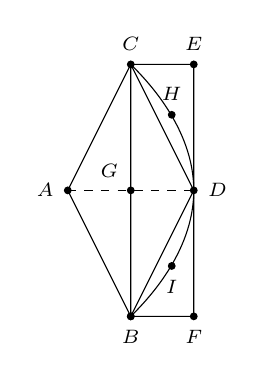
\begin{tikzpicture}[scale=.8]
			\draw[] (0,0)node[circle,fill,inner sep = 1,label = below:\scriptsize$B$]{}--(1,0)node[circle,fill,inner sep=1pt,label = below:\scriptsize$F$]{}--(1,2)node[circle,fill,inner sep=1pt,label = right:\scriptsize$D$]{}--(1,4)node[circle,fill,inner sep=1pt,label = above:\scriptsize$E$]{}--(0,4)node[circle,fill,inner sep=1pt,label = above:\scriptsize$C$]{}--(-1,2)node[circle,fill,inner sep=1pt,label = left:\scriptsize$A$]{}--(0,0)node[circle,fill,inner sep=1pt]{}--(0,2)node[circle,fill,inner sep=1pt,label = above left:\scriptsize$G$]{}--(0,4)--(1,2)--(0,0);
			\draw[dashed](-1,2)--(1,2);
			\draw[rotate=90] (0,0) parabola bend (2,-1) (4,0);
			\draw[] (.65,.8)node[circle,fill,inner sep = 1,label = below:\scriptsize$I$]{};
			\draw[] (.65,3.2)node[circle,fill,inner sep = 1,label = above:\scriptsize$H$]{};
		    \end{tikzpicture}
		\end{center}
		\vspace{.5cm}
		$CB$ es arista de $P$ mientras $CD$ y $DB$ son aristas de $P^{'}$. Sea $a$ la diferencia entre las áreas del sector circular $AIDHCA$ y la parte del polígono $P$ que se encuentra dentro de este sector, De este modo,
		$$a=Area(ABIDHCA)-Area(\triangle CAB) = Area(CGBIDHC)$$
		Sea $b$ la diferencia entre las áreas del sector circular $ABIDHCA$ y la parte del polígono $P^{'}$ que se encuentra dentro de este sector, De este modo,
		$$b=Area(ABIDHCA)-Area(\square CABD) = Area(DBID)+Area(CDHC)$$
		Donde demostraremos que $b\leq \dfrac{a}{2}.$
		$$b\leq \dfrac{a}{2}\; \Leftrightarrow \; -b\geq a-b\geq a-\dfrac{a}{2}\; \Leftrightarrow \; a-b\geq \dfrac{a}{2}.$$
		Por lo tanto probaremos la equivalencia $a-b\geq \dfrac{a}{2}.$

		$$\begin{array}{rcl}
		    a-b&=&Area(CGBIDHC)-\left[Area(DBID)+Area(CDHC)\right]\\\\
		       &=&Area(\triangle CBD)\\\\
		       &=&Area(\triangle CGD)+Area(\triangle BGD) \qquad \mbox{ ya que } \triangle BGD \cong \triangle CED\\\\
		       &=&Area(\triangle CGD)+Area(\triangle CED)\\\\
		       &=&Area(\square CGDE)\\\\
		\end{array}$$

		$$\begin{array}{rcl}
		    a&=&Area(CGDIBHC)\\\\
		     &=&Area(CGDHC)+Area(GBIDG)\\\\
		     &=&2Area(CGDHC)\qquad \mbox{ ya que } CGDHC \cong GBIDG\\\\
		\end{array}$$

		Así
		$$\dfrac{1}{2}=Area(CGDHC)$$

		Observe que $CGDHC$ es contenido en $\square$, de donde $Area(CGDHC)\leq Area(\square CGDE)$, comparando las inecuaciones $Area(\square CGDE)$ y $\dfrac{a}{2}=Area(CGDHC)$ tenemos,
		$$a-b\geq \dfrac{a}{2}.$$\\


	    %---------- (c)
	    \item Demuestre que existe un polígono regular $P$ inscrito en un círculo y con área tan próxima como se desee al área del círculo.\\\\
		Demostración.-\; Supongamos $P_1$ un triángulo equilátero inscrito en una circunferencia y sea $P_n$ el polígono regular con lados $3\cdot 2^n$ inscrito en el mismo circo. Luego sea $a_n$ denotado por la diferencia entre el área del circulo y la de $P_n$. Entonces por la parte (b),
		$$a_{n+1}\leq \dfrac{a_n}{2}$$
		Por la parte (a), dado cualquier $\epsilon$, podemos encontrar $n$ tal que $a_n<\epsilon$. Esto es, dado cualquier $\epsilon,$ se tiene $P_n$ tal que la diferencia entre el área del circulo y la del $P_n$ es menor que $\epsilon.$\\
		En otras palabras, podemos encontrar $P_n$ cuya área es tan cercana al área del circulo como se desee.\\\\

	    %---------- (d)
	    \item Utilizando el hecho de que las áreas de dos polígonos regulares con el mismo número de lados están entre sí en la misma relación que los cuadrados de sus lados, demuestre que las áreas de dos círculos están en la misma relación que los cuadrados de sus radios.\\\\
		Demostración.-\; Consideremos dos círculos $C_1$ y $C_2$ co radio $r_1$ y $r_2$ respectivamente. Asumamos que 
		$$\dfrac{Area C_1}{Area C_2} = R< \dfrac{r^2_1}{r^2_2}$$
		Elijase $\epsilon>0$ tal que $R<R+\epsilon < \dfrac{r_1^2}{r^2_2}$. Se tiene un polígono regular de n lado en $C_1$ y $C_2$. Llamados $P_1$ y $P_2$ respectivamente. Sea las longitudes de estos lados $d_1$ y $d_2$. Entonces,
		$$d_1 = 2r_1\sen(\pi/n), \qquad d_2 = 2r_2\sen(\pi/n)$$
		Por lo tanto, $\dfrac{d_1^2}{d_2^2}=\dfrac{r_1^2}{r_2^2}=R.$
		Asumimos que $Area C_1=Area P_1 + \epsilon_1$ y $Area C_2 = Area P_2+\epsilon_2.$\\
		Para $\dfrac{Area C_1}{Area C_2} = R< \dfrac{r^2_1}{r^2_2}$ obtenemos,
		$$Area C_1 = R\cdot Area C_2$$
		así,
		$$Area P_1 + \epsilon_1 = R(Area P_2 + \epsilon_2)\; \Rightarrow \; \dfrac{Area P_1}{Area P_2}=R+\dfrac{1}{Area P_2}(R \epsilon_2 + \epsilon_1)$$
		Demostramos que podemos elegir $n$ suficiente grande tal que $\epsilon_1$ y $\epsilon_2$ puede ser tan pequeño como se desee. Ahora elijamos $n$ tal que $\dfrac{1}{Area P_2}(R \epsilon_2 - \epsilon_1)<\epsilon.$ Entonces 
		$$\dfrac{Area P_1}{Area P_2}=R+\dfrac{1}{Area P_2}(R \epsilon_2-\epsilon_1)<R+\epsilon < \dfrac{r^2_1}{r^2_2}=\dfrac{d_1^2}{d_2^2}$$
		donde $\dfrac{Area P_1}{Area P_2}<\dfrac{d_1^2}{d_2^2}$ es una contradicción ya que ambos $P_1$ y $P_2$ son polígonos regulares que tiene igual número de lados. Esto muestra que nuestra suposición inicial $\dfrac{Area C_1}{Area C_2}<\dfrac{r_1^2}{r_2^2}$ es incorrecto. Por otro lado podemos argumentar análogamente y llegar a una contradicción si asumimos $\dfrac{Area C_1}{Area C_2}>\dfrac{r_1^2}{r_2^2}$. Así se sigue,
		$$\dfrac{Area C_1}{Area C_2}=\dfrac{r_1^2}{r_2^2}.$$\\

	\end{enumerate}

    %-------------------- 12
    \item Supongamos que $A$ y $B$ son dos conjuntos no vacíos de números tales que $x\leq y$ para todo $x$ en $A$ y todo $y$ de $B$.

	\begin{enumerate}[\bfseries (a)]

	    %---------- (a)
	    \item Demuestre que $\sup A \leq y$ para todo $y$ de $B$.\\\\
		Demostración.-\; Puesto que cualquier $y$ en $B$ satisface $y\geq x$ para todo $x$ en $A$, cualquiera $y$ en $B$ es una cota superior de $A$, por tanto $y\geq \sup A$.\\\\ 

	    %---------- (b)
	    \item Demuestre que $\sup A \leq \inf B.$\\\\
		Demostración.-\; El apartado (a) demuestra que $\sup A$ es una cota inferior de $B$, por tanto $\sup A \leq \inf B.$\\\\

	\end{enumerate}

    %-------------------- 13
    \item Sean $A$ y $B$ dos conjuntos numéricos no vacíos y acotados superiormente, y sea $A+B$ el conjunto de todos los números $x+y$ con $x$ de $A$ e $y$ de $B$. Demuestre que $\sup(A+B)=\sup A + \sup B$.\\\\
	Demostración.-\; Supuesto que $x\leq \sup A$ e $y\leq \sup B$ para cualquier $x$ en $A$ e $y$ en $B$, se deduce que $x+y\leq \sup A + \sup B$. En consecuencia, $\sup A + \sup B$ es una cota superior de $A+B$, por tanto $$\sup(A+B)\leq \sup A + \sup B.$$
	Para todo $\epsilon>0$. Ya que $\sup A$ es una cota superior mínima de $A$ y $\sup A - \epsilon/2$ no es una cota superior de $A$, entonces existe un $x\in A$ tal que $\sup A-x<\epsilon/2$. De similar forma, existe un $y\in B$ tal que $\sup B - y < \epsilon/2.$ Así nos aseguramos que $\sup A + \sup B>(x+y)$, es decir,
	$$\sup A + \sup B - (x+y)<\epsilon$$
	Luego por hipótesis sabemos que,
	$$\sup(A+B)\geq x+y$$
	de donde,
	$$\sup(A+B)\geq x+y>\sup A + \sup B - \epsilon$$

	Por lo tanto, $\sup(A+B)=\sup A + \sup B$.\\\\

    %-------------------- 14
    \item 
	\begin{enumerate}[\bfseries (a)]

	    %---------- (a)
	    \item Considere una sucesión de intervalos cerrados $I_1 = [a_1,b_1],\; I_2 = [a_2,b_2], \ldots$. Suponga que $a_n\leq a_{n+1}$ y que $b_{n+1}\leq b_n$ para todo $n$. Demuestre que existe un punto $x$ que pertenece a todos los $I_n$.\\\\
	    \begin{center}
	    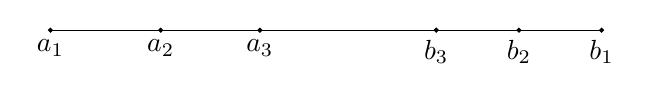
\begin{tikzpicture}[scale=.7]
		\draw[] (0,0)--(10,0);
		\filldraw[black] (0,0) circle (1pt) node[below]{$a_1$};
		\filldraw[black] (2,0) circle (1pt) node[below]{$a_2$};
		\filldraw[black] (3.8,0) circle (1pt) node[below]{$a_3$};
		\filldraw[black] (7,0) circle (1pt) node[below]{$b_3$};
		\filldraw[black] (8.5,0) circle (1pt) node[below]{$b_2$};
		\filldraw[black] (10,0) circle (1pt) node[below]{$b_1$};
	    \end{tikzpicture}
	    \end{center}
		Demostración.-\; 

	    %---------- (b)
	    \item Demuestre que esta conclusión es falsa si se consideran intervalos abiertos en lugar de intervalos cerrados.\\\\
		Demostración.-\;
		El sencillo resultado del problema 14(a) se denomina Teorema de los Intervalos Encajados. Puede utilizarse para dar otras demostraciones de los Teoremas 1 y 2. El procedimiento utilizado, que se ilustra en los dos problemas siguientes, ilustra un método general denominado argumento de bisección.\\\\

	\end{enumerate}

    %-------------------- 15
    \item Suponga que $f$ es continua en $[a,b]$ y $f(a)<0<f(b)$. Entonces o bien $f[(a+b)/2] = 0$, o $f$ tiene signos distintos en los extremos del intervalo $[a,(a+b)/2]$, o bien $f$ tiene distintos en los extremos del intervalo $[(a+b)/2,b]$. ¿Por qué? Si $f[(a+b)/2]\neq 0$, sea $I_1$ aquel de los dos intervalos en el que $f$ cambia de signo. Divida ahora $I_1$ en dos mitades. O bien $f$ en $0$ en el punto medio, o bien $f$ cambia de signo en uno de los dos intervalos. Sea $I_2$ uno de estos. Continue de esta manera definiendo $I_n$ para cada $n$ (a no ser que $f$ sea $0$ en algún punto medio). Utilice el teorema de los intervalos encajados para hallar un punto $x$ en el que $f(x)=0$.\\\\
	Demostración.-\; Si $f$ es cero en algún punto medio, entonces quedará demostrada la proposición. Supongamos que $f$ no es cero en ningún punto medio. Si denotamos el n-simo intervalo por $I_n=[a_n,b_n]$, podemos seguir construyendo $I_n$ indefinidamente. Esta $I_n$ tendrá la siguientes propiedades.
	\begin{enumerate}[(a)]
	    \item $[a,b] = I_0 \supseteq I_1 \supseteq I_2 \supseteq \ldots$
	    \item $l(I_n) = \dfrac{1}{2} l(I_n)$ donde $l(I)$ denota la longitud del intervalo $I$.
	\end{enumerate}

	Por el argumento del ejercicio anterior, tenemos $a_m\leq b_n$ para todo $m$ y $n$, que demuestra que el conjunto $A=\lbrace a_m : m\in \mathbb{N} \rbrace$ es acotado superiormente y cada $b_n$ es una cota superior de $A$. Sea $x=\sup A$, entonces $a_n\leq x$ para cada $n\geq 0$ y ya que $x$ es la mínima cota superior, tenemos también $x\leq b_n$ para cada $n\geq 0$. De donde 
	$$a_n\leq x \leq b_n$$
	para cada $n$.\\
	Similarmente, el conjunto $B=\lbrace b_n : n\in \mathbb{N} \rbrace$ es acotado superiormente y cada $a_m$ es una cota inferior de $B$. Sea $y=\inf A$, entonces $b_n\geq y$ para cada $n\geq 0$ y ya que $y$ es la mayor cota inferior, tenemos también $y\geq a_n$ para cada $n\geq 0$ y por lo tanto,
	$$a_n\leq y \leq b_n$$
	para cada $n$.\\
	Si $x\leq z \leq y,$ entonces $a_n\leq x \leq z \leq y \leq b_n$ para cada $n$. Por lo tanto, el intervalo $[x,y]$ se encuentra en $I_n$, para cada $n$. Esto es,
	$$[x,y]\subseteq \bigcap_{n=0}^{\infty} I_n$$
	Recordemos la segunda propiedad citada a un principio. Usando recursivamente tenemos lo siguiente,
	$$l(I_n) = \dfrac{1}{2}l \left(I_{n-1}\right) = \left(\dfrac{1}{2}\right)^2 l\left(I_{n-2}\right) = \ldots = \left(\dfrac{1}{2}\right)^nl(I_0) = \dfrac{b-a}{2^n}$$
	Esto muestra que $l(I_n)\to 0$ cuando $n\to \infty$. Ya que $\displaystyle\bigcap_{n=0}^{\infty} I_n \subseteq I_n$ para cada $n$, tenemos $[x,y]\subseteq I_n$ para cada $n$.\\
	Como $n\to \infty$ entonces $l(I_n)\to 0$, efectivamente $l([x,y])=0$. Esto será posible si y sólo si $x=y.$ Esto implica que $\displaystyle\bigcap_{n=0}^\infty I_n$ consiste de un simple elemento
	$$\bigcap_{n=0}^\infty I_n = {x}$$
	Ahora probemos que para este $x, f(x)=0$. Tenemos $\sup A = x = y = \inf B$. Ya que $(a_n)$ es una secuencia creciente, $a_n\to x.$ Similarmente, $b_n\to x.$ Esto implica que $f(a_n)\to f(x)$ y $f(b_n) \to f(x)$ esto como $f$ es continuo. Sin embargo, por construcción $f(a_n)<0$ para todo $k$ y $f(b_n)>0$ para todo $k$. Esto es $f(x)$ tiene dos sucesiones, una formada por números positivos y la otra por números negativos, que convergen en ella. Esto es posible si $f(x)=0.$\\\\

    %-------------------- 16.
    \item Suponga que $f$ es continua en $[a,b]$, pero que no estuviese acotada en $[a,b]$. Entonces $f$ no estaría acotada en $[a,(a+b)/2]$ o bien no lo estaría en $[(a+b)/2,b]$. ¿Por qué? Sea $I_1$ uno de estos intervalos en los que $f$ no está acotada. Aplique el método utilizado en el problema 15 para llegar a una contradicción.\\\\
	Demostración.-\; Si denotamos el n-esimo intervalo por $I_n=[a_n,b_n]$ podemos seguir construyendo $I_n$ indefinidamente. Esta $I_n$ satisfacerá las siguientes propiedades.
	\begin{enumerate}[(a)]
	    \item $[a,b] = I_0 \supseteq I_1 \supseteq I_2 \supseteq \ldots$
	    \item $l(I_n) = \dfrac{1}{2} l(I_n)$ donde $l(I)$ denota la longitud del intervalo $I$.
	\end{enumerate}
	Por el argumento del anterior ejercicio, tenemos $a_m\leq b_n$ para cada $m$ y cada $n$. Esto demuestra que el conjunto $A=\left\{a_m : m\in \mathbb{N}\right\}$ es acotado superiormente y cada $b_n$ es un una cota superior de $A$. Luego sea $x=\sup A$, entonces $a_n\leq x$ para cada $n\geq 0$ y ya que $x$ es la mínima cota superior, tenemos también $x\leq b_n$ para cada $n\geq 0$. De donde 
	$$a_n\leq x \leq b_n$$
	para cada $n$.\\
	Similarmente, el conjunto $B=\lbrace b_n : n\in \mathbb{N} \rbrace$ es acotado superiormente y cada $a_m$ es una cota inferior de $B$. Sea $y=\inf A$, entonces $b_n\geq y$ para cada $n\geq 0$ y ya que $y$ es la mayor cota inferior, tenemos también $y\geq a_n$ para cada $n\geq 0$ y por lo tanto,
	$$a_n\leq y \leq b_n$$
	para cada $n$.\\
	Si $x\leq z \leq y,$ entonces $a_n\leq x \leq z \leq y \leq b_n$ para cada $n$. Por lo tanto, el intervalo $[x,y]$ se encuentra en $I_n$, para cada $n$. Esto es,
	$$[x,y]\subseteq \bigcup_{n=0}^{\infty} I_n$$
	Recordemos la segunda propiedad citada a un principio. Usando recursivamente tenemos lo siguiente,
	$$l(I_n) = \dfrac{1}{2}l \left(I_{n-1}\right) = \left(\dfrac{1}{2}\right)^2 l\left(I_{n-2}\right) = \ldots = \left(\dfrac{1}{2}\right)^nl(I_0) = \dfrac{b-a}{2^n}$$
	Esto muestra que $l(I_n)\to 0$ cuando $n\to \infty$. Ya que $\displaystyle\bigcap_{n=0}^{\infty} I_n \subseteq I_n$ para cada $n$, tenemos $[x,y]\subseteq I_n$ para cada $n$.\\
	Como $n\to \infty$ entonces $l(I_n)\to 0$, efectivamente $l([x,y])=0$. Esto será posible si y sólo si $x=y.$ Esto implica que $\displaystyle\bigcap_{n=0}^\infty I_n$ consiste de un simple elemento
	$$\bigcap_{n=0}^\infty I_n = {x}$$
	Ya que $f$ no está acotado en cada $I_n$ y cada $x$ se encuentra en cada $I_n$, entonces $f$ no está acotado en $x$. De donde llegamos a una contradicción ya que por hipótesis $f$ no está acotada en $[a,b]$.\\\\

    %-------------------- 17.
    \item 
	\begin{enumerate}[(a)]

	    %----------(a)
	    \item Sea $A=\left\{x:x<\alpha \right\}$. Demuestre lo siguiente:

		\begin{enumerate}[(i)]

		    %----- (i)
		    \item Si $x$ pertenece a $A$ e $y<x$, entonces $y$ pertenece a $A$.\\\\
			Demostración.-\; Que $x$ esté en $A$ implica que $x<\alpha$, luego que $y<x$ implica que $y<x<\alpha$. De este modo $y \in A$.\\\\

		    %----- (ii)
		    \item $A\neq \emptyset$.\\\\
			Demostración.-\; Que $\alpha-1<\alpha$ implica que $\alpha-1\in A$, por lo que $A\neq \emptyset$.\\\\

		    %----- (iii)
		    \item $A\neq \mathbb{R}$.\\\\
			Demostración.-\; Análogo al anterior inciso, se tiene que $\alpha + 1>\alpha$ que implica que $\alpha +1 \notin A,$ por lo que $A\neq \mathbb{R}.$\\\\

		    %----- (iv)
		    \item Si $x$ pertenece a $A$, entonces existe algún número $x^{'}$ de $A$ tal que $x<x^{'}$.\\\\
			Demostración.-\; Sea $x\in A$, entonces $x<\alpha$ de donde $\alpha-x>0$, luego sea $x^{'}=x+\dfrac{\alpha-x}{2}$, entonces $x^{'}>x$ ya que $\dfrac{\alpha-x}{2}>0$, por lo tanto
			$$x^{'}=x+\dfrac{\alpha-x}{2}=\dfrac{\alpha+x}{2}<\dfrac{\alpha+\alpha}{2}=\alpha.$$
			Esto demuestra que $x^{'}<\alpha$ lo que implica que $x^{'}\in A.$\\\\

		\end{enumerate}

		%----------(b)
	    \item Suponga a la inversa, que $A$ satisface (i)-(iv). Demuestre que $A=\left\{x:x<\sup A\right\}$.\\\\
		Demostración.-\; Supongamos que $z\in \mathbb{R}$ tal que $z\notin A$. Luego sea $x>z$, si $x\in A$, entonces por la propiedad (i), $z$ también está en $A$, lo que contradice el hecho de que $z\notin A.$ Lo que demuestra que $A$ está acotado superiormente por $z$. Luego ya que $A\neq \emptyset$ entonces el $\sup A$ existe. Por último, dado que $x\in A$, elíjase $x^{'}$ en $A$, de donde según (iv), con $x<x^{'}$, entonces $x<x^{'}\leq \sup A$, con lo que $x<\sup A$. Recíprocamente, si $x<\sup A$, existe entonces un $y$ en $A$ con $x<y$. De aquí, por (i), $x\in A.$\\\\

	\end{enumerate}

    %-------------------- 18.
    \item Un número $x$ se denomina una casi cota superior de $A$ si en $A$ existen sólo un número finito de números $y$ con $y\geq x.$ Del mismo modo se define una casi cota inferior de $A$.

	\begin{enumerate}[(a)]

	    %----------(a)
	    \item Halle todas las casi cotas superiores y todas las casi cotas inferiores de los conjuntos del problema 1.\\\\

		Respuesta.-\; \\ 
		\begin{enumerate}[(i)]

		    %----- (i)
		    \item Llamemos al conjunto de cotas casi superiores del conjunto $A$ con $csup A$, y el conjunto de cotas casi inferiores con $cinf A$, entonces tenemos
		    $$A=\left\{\dfrac{1}{n} : n\in \mathbb{N}\right\}=\left\{1,\dfrac{1}{2},\dfrac{1}{3},\dfrac{1}{4},\ldots\right\}$$
		    de donde cualquier cota casi superior es una cota superior (cero elementos $y$ tal que $y\geq x$ son un número finito de elementos) por lo que $[1,\infty) \subseteq csup A$. Luego cada número positivo $\epsilon$ es una cota casi superior, ya que $\dfrac{1}{n}>\epsilon$ tiene un número finito de soluciones ($\frac{1}{n}< \epsilon \Rightarrow n < \frac{1}{\epsilon}$ número finito de soluciones para $\epsilon$). Sabemos que cero o cualquier número negativo $x$, no es una cota casi superior, ya que existe infinitos elementos del conjunto $A$ tal que $\dfrac{1}{n}\geq 0$ o $\dfrac{1}{n}\geq x$. Así,
		    $$csup A = (0,\infty)$$
		    Por otro lado cualquier cota inferior es una cota casi inferior (cero elementos $y$ tal que $y\leq x$ son un número finito de elementos) entonces $(-\infty,0]\subseteq cinf A$. Ningún elementos positivo $x$ es una cota casi inferior, ya que existe infinitos elementos del conjunto $A$ tal que $\dfrac{1}{n}\leq x$. Así,
		    $$cinf A = (-\infty,0].$$\\

		    %----- (ii)
		    \item Sea
		    $$A=\left\{\dfrac{1}{n} : n\in \mathbb{Z},\; n\neq 0\right\} = \left\{1,-1,\dfrac{1}{2},-\dfrac{1}{2},\dfrac{1}{3},-\dfrac{1}{3},\ldots\right\}$$
		    De donde cualquier cota casi superior es una cota superior (cero elementos $y$ tal que $y\geq x$ son un número finito de elementos) por lo que $[1,\infty) \subseteq csup A$. Luego cada número positivo $\epsilon$ es una cota casi superior, ya que $\dfrac{1}{n}>\epsilon$ tiene un número finito de soluciones ($\frac{1}{n}< \epsilon \Rightarrow n < \frac{1}{\epsilon}$ número finito de soluciones para $\epsilon$). Sabemos que cero o cualquier número negativo $x$, no es una cota casi superior, ya que existe infinitos elementos del conjunto $A$ tal que $\dfrac{1}{n}\geq 0$ o $\dfrac{1}{n}\geq x$. Así,
		    $$csup A = (0,\infty)$$
		    Por otro lado cada número negativo $V$ es una cota casi superior, ya que existe un finito número $y$ de elementos del conjunto $A$ tal que $y\leq V$. Sabemos que cero o cualquier número negativo $x$, no es una cota casi inferior, ya que existe infinitos elementos del conjunto $A$ tal que $y\leq x$. Así,
		    $$cinf A = (-\infty,0].$$\\

		    %----- (iii)
		    \item Similar a los anteriores incisos,
			$$csup A = (0,\infty),\qquad cinf A = (-\infty,0].$$\\

		    %----- (iv)
		    \item $$csup A = [\sqrt{2},\infty],\qquad cinf A = (-\infty,0].$$\\

		    %----- (v)
		    \item $$\left\{ x: x^2 + x + 1 \geq 0 \right\}=\mathbb{R}$$
			La desigualdad se cumple para todos los números reales, por lo que no hay una cota casi superior, ni una cota casi inferior.\\\\

		    %----- (vi)
		    \item Se tiene,
			$$x^2+x-1=0\quad \Rightarrow \quad x_{1,2} = \dfrac{-1\pm \sqrt{1^2+4}}{2} \quad \Rightarrow \quad x_1 = -\dfrac{1}{2}-\dfrac{\sqrt{5}}{2},\quad x_2=-\dfrac{1}{2}+\dfrac{\sqrt{5}}{2}.$$
			La parabola está abierta hacia arriba, entonces el conjunto solución es un intervalo 
			$$\left(-\dfrac{1}{2}-\dfrac{\sqrt{5}}{2}, -\dfrac{1}{2}+\dfrac{\sqrt{5}}{2}\right)$$
			Así,
			$$csup A = \left[-\dfrac{1}{2}-\dfrac{\sqrt{5}}{2},\infty\right),\qquad cinf A = \left(-\infty,-\dfrac{1}{2}+\dfrac{\sqrt{5}}{2}\right].$$\\

		    %----- (vii)
		    \item $$A=\left\{x:x<0 \; \land \; x-1<0\right\}=\left(-\dfrac{1}{2}-\dfrac{\sqrt{5}}{2},0\right)$$
			Así,
			$$csup A = [0,\infty), \quad cinf = \left(-\infty,-\dfrac{1}{2}-\dfrac{\sqrt{5}}{2}\right].$$\\

		    %----- (viii)
		    \item $$A=\left\{\dfrac{1}{n} + (-1)^n:n\in \mathbb{N}\right\}$$
			La subsecuencia con índices impares converge a $-1$, mientras que la subsecuencia con índices pares converge a 1, por lo que hay infinitos elementos del conjunto $A$ entre $1$ y $-1$, por lo tanto
			$$csup A = (1,\infty),\qquad cinf A  = (-\infty,-1].$$\\

		\end{enumerate}


	    %----------(b)
	    \item Suponga que $A$ es un conjunto finito acotado, Demuestre que el conjunto $B$ de todas las casi cotas superiores de $A$ es no vacío y está acotado inferiormente.\\\\
		Demostración.-\; Dado que $A$ está acotado, tiene al menos una cota superior, y ese también es una cota casi superior, por lo que el conjunto $B$ de cotas casi superiores no está vacío. Además, dado que $A$ está acotado, tiene al menos una cota  inferior, digamos $l$. Debido a que $A$ es infinito, hay infinitos elementos de $A$ por encima de $l$, por lo que $l$ no es una casi cota superior, y tampoco lo es ningún número debajo de $l$, por la misma razón. Por lo tanto, $l$ es una cota inferior para el conjunto de todos los límites casi superiores, y $B$ está ciertamente acotado por abajo.\\\\

	    %----------(c)
	    \item Del apartado (b) se deduce que existe el $\inf B$; este número se denomina el límite superior de $A$, y se representa mediante el símbolo $\overline{\lim} A$ o $\lim A$ para cada conjunto $A$ del problema 1.\\\\
		Respuesta.-\; Por (a) se sigue,
		\begin{enumerate}[(i)]
		    
		    %----- (i)
		    \item $\overline{\lim} A = 0$.\\\\

		    %----- (ii)
		    \item $\overline{\lim} A = 0$.\\\\

		    %----- (iii)
		    \item $\overline{\lim} A = 0$.\\\\

		    %----- (iv)
		    \item $\overline{\lim} A = \sqrt{2}$.\\\\

		    %----- (v)
		    \item No existe.\\\\

		    %----- (vi)
		    \item $\overline{\lim} A = -\dfrac{1}{2}+\dfrac{\sqrt{5}}{2}$.\\\\

		    %----- (vii)
		    \item $\overline{\lim} A = 0$.\\\\

		    %----- (viii)
		    \item $\overline{\lim} A = 1$.\\\\

		\end{enumerate}

	    %----------(d)
	    \item Defina el $\underline{\lim} A$ y hállelo para todos los $A$ del problema 1.\\\\
		Respuesta.-\; Si $A$ es un conjunto infinito acotado, existe números $m$ y $M$ tal que
		$$m\leq y \leq M,\; \forall \; y \in A$$
		Luego, $m$ es una cota casi inferior de $A$ ya que o no existe elemento $y$ de $A$ tal que $y\leq M$ o existe un elemento $y=M$ de $A$ tal que $y\leq M$. Denotemos el conjunto de todas las cotas casi inferiores de $A$ con $C$. Este último conjunto está acotado superiormente con $M$, llamemos a este número cota inferior de $A$ y denotado por $\underline{\lim} A$. Se sigue de (a):\\

		\begin{enumerate}[(i)]

		    %----- (i)
		    \item $\underline{\lim} A = 0$.\\\\

		    %----- (ii)
		    \item $\underline{\lim} A = 0$.\\\\

		    %----- (iii)
		    \item $\underline{\lim} A = 0$.\\\\

		    %----- (iv)
		    \item $\underline{\lim} A = 0$.\\\\

		    %----- (v)
		    \item No existe.\\\\

		    %----- (vi)
		    \item $\underline{\lim} A = -\dfrac{1}{2}-\dfrac{\sqrt{2}}{2}$.\\\\

		    %----- (vii)
		    \item $\underline{\lim} A = -\dfrac{1}{2}-\dfrac{\sqrt{5}}{2}$.\\\\

		    %----- (viii)
		    \item $\underline{\lim} A = -1$.\\\\

		\end{enumerate}

	\end{enumerate}

    %-------------------- 19.
    \item Si $A$ es un conjunto infinito acotado demuestre que

	\begin{enumerate}[(a)]

	    %----------(a)
	    \item $\underline{\lim} A \leq \overline{\lim} A.$\\\\
		Demostración.-\; Sea $B$ el conjunto de cotas casi superiores de $A$, entonces $\overline{\lim} A = \inf B.$ Por la propiedad de infimo, existe $\alpha<\overline{\lim} A + \epsilon$ tal que $\alpha \in B$. Por lo que existe un número finito de elementos de $A$ mayores o iguales a $\alpha.$ Por otro lado sea $C$ el conjunto de cotas casi inferiores de $A$, entonces $\underline{\lim} A = \sup C$. Por la propiedad de supremo, existe $\beta>\underline{\lim} A - \epsilon$ tal que $\beta \in C$. Por lo tanto existe un número finito de elementos de $A$ menores o iguales que $\beta$.\\
		Ahora, probemos que $\beta<\alpha$. Sea $\beta\geq \alpha,$ ya que existe un número finito de elementos de $A$ mayores o iguales que $\alpha$, entonces $\beta\geq \alpha$ implica que existe finitos números de $A$ mayores o iguales a $\beta$. Sin embargo, existe números finitos elementos de $A$ mayores o iguales que $\beta\in C$. Esto significa que existe número finitos elementos en $A$ lo que contradice la hipótesis de que $A$ es infinito. De este modo $\beta<\alpha$ implica que $\underline{\lim} A -\epsilon < \beta < \alpha < \overline{\lim} A + \epsilon.$ Que $\underline{\lim} A - \epsilon < \overline{\lim} A + \epsilon$ para cada $\epsilon>0$ implica que $\underline{\lim} A \leq \overline{\lim} A.$\\\\

	    %----------(b)
	    \item $\overline{\lim} A \leq \sup A$.\\\\
		Demostración.-\; Si $B$ denota el conjunto de cotas casi superiores de $A$, entonces $\sup A \in B$. Luego ya que $\overline{\lim} A = \inf B,$ por lo propiedad de ínfimo, $\overline{\lim} \leq \sup A$.\\\\

	    %----------(c)
	    \item Si $\overline{\lim} A < \sup A$, entonces $A$ contiene un elemento máximo.\\\\
		Demostración.-\; Sea $\overline{\lim} A < \sup A,$ elija $z$ tal que $\overline{\lim} < z < \sup A$. Si $B$ es el conjunto de cotas casi superiores de $A$, entonces $z\in B.$ Por lo tanto existe un número finito de elementos de $A$ mayores o iguales que $z$. Por otro lado, ya que $z<\sup A$, existe al menos un elementos de $A$ mayores o iguales a $z$. Es decir, hay un número finito y diferentes de cero en $A$ mayor o igual que $z$, donde se elije el elemento más grande de $A$.\\\\

	    %----------(d)
	    \item Demuestre los casos análogos a los apartados (b) y (c) para $\underline{\lim}$.\\\\
		Demostración.-\; Probemos que $\underline{\lim} A \geq \inf A.$ Si $C$ denota el conjunto de cotas casi superiores de $A$, entonces $\inf A \in C$. Ya que $\underline{\lim} A = \sup B$, por la propiedad de supremo $\underline{\lim} A \geq \inf A$. \\
		Ahora demostremos que si $\underline{\lim} A  > \inf A$, entonces $A$ contiene el elemento más pequeño. Asumiendo que $\underline{\lim} A > \inf A$, elija $z$ tal que $\underline{\lim} A > z > \inf A$. Si $C$ es el conjunto de cotas casi inferiores de $A$, entonces $z\in C$. Por lo tanto existe números finitos de elementos de $A$ menores o iguales que $z$. Por otro lado, ya que $z>\inf A$, existe al menos un elemento de $A$ menores o iguales que $z$. Es decir, existe un número diferente de cero y finito de $A$ mejor o igual que $z$. Donde se elije al elemento más pequeño de $A$.\\\\  

	\end{enumerate}

    %-------------------- 20.
    \item Sea $f$ una función continua en $\mathbb{R}$. Un punto $x$ se denomina un punto de sombra de $f$ si existe un número $y>x$ con $f(y)>f(x)$. Suponga que todos los puntos de $(a,b)$ son puntos de sombra, pero que $a$ y $b$ no lo son. En este caso se verifica, evidentemente, que $f(a)\geq f(b).$

	\begin{enumerate}[(a)]

	    %----------(a)
	    \item Suponga que $f(a)>f(b)$. Demuestre que el punto en el que $f$ alcanza su valor máximo en $[a,b]$ ha de ser $a$.\\\\
		Demostración.-\; Supongamos que $f(a)>f(b)$, de donde debemos demostrar que $f$ tiene un valor máximo en el punto $a$ del intervalo $[a,b]$. Sea $z\in (a,b]$ un punto el cual la función alcanza su máximo. Por lo que tenemos que $f(z)>f(x),\; \forall \; x\in (a,b]$. Pero, $z$ es el punto de sombra por la suposición inicial. Esto significa que existe algún punto $z^{'}$ por el cual $f(z)<f(z^{'})$. Este punto no puede estar en el intervalo $(a,b)$ ya que $f(z)$ es el máximo en el intervalo. De aquí se sigue que $z^{'}>b$. De donde la combinación de todos estos resultados da,
		$$f(b)<f(z)\leq f(z^{'}), \mbox{ para } b<z^{'}$$
		Por lo tanto, $b$ no es el punto de sombra, así demostramos que es una contradicción. Se sigue que $z=a$, es decir, la función debe alcanzar su máximo en el punto $a$.\\\\

	    %----------(b)
	    \item Demuestre ahora que esto conduce a una contradicción, de manera que se ha de verificar que $f(a)=f(b).$\\\\
		Demostración.-\; Existe tres posibilidades para $f(a)$ y $f(b)$. 
		$$f(a)<f(b),\quad f(a)>f(b) \quad \mbox{o} \quad f(a)=f(b).$$
		Supongamos que $f(a)<f(b)$, ya que $a<b$, de la definición de los puntos de sombra se sigue que $a$ será el punto de sombra, el cual es una contradicción.\\
		Supongamos ahora que $f(a)>f(b)$, de donde sabemos que todos los puntos $x\in (a,b)$ son puntos de sombra, mientras $b$  no es un punto de sombra. Por lo tanto $f(x)<f(b)$ para todo $x\in (a,b)$. Sabemos que $f$ es una función continua, de la deducción anterior se sigue que existirá algún punto $t\in (a,b)$ por el cual $f(t)=f(b).$\\
		Ya que $b$ no es un punto de sombra, entonces $f(b)>f(x)$ para $x>b$. Tengamos en cuenta que no es difícil deducir que $f(t)>f(x),\; \forall\; x > b$. Por lo tanto, los puntos en el intervalo $(a,t)$ no son puntos de sombra, ya que $f(t)<f(z),\; \forall\; z \in (a,t)$. Esto es también contradictorio. Por lo que $f(a)=f(b)$.\\\\

	\end{enumerate}

\end{enumerate}

\section{Apéndice: Continuidad Uniforme}

\begin{tcolorbox}
    \begin{def.}
	La función $f$ es uniformemente continua en un intervalo $A$ si para cada $\epsilon>0$ existe algún $\delta>0$ tal que, para todo $x$ e $y$ de $A$,
	\begin{center}
	    $|x-y|<\delta,$ entonces $|f(x)-f(y)|<\epsilon.$
	\end{center}
    \end{def.}
\end{tcolorbox}

\begin{lema}
    Sea $a<b<c$ y $f$ continua en el intervalo $[a,c]$. Sea $\epsilon>0$ y supongamos que si verifican,
    \begin{enumerate}[(i)]
	\item Si $x$ e $y$ pertenecen a $[a,b]$ y $|x-y|<\delta_1$ entonces $|f(x)-f(y)|<\epsilon,$
	\item Si $x$ e $y$ pertenecen a $[b,c]$ y $|x-y|<\delta_2$ entonces $|f(x)-f(y)|<\epsilon.$
    \end{enumerate}
    Entonces existe un $\delta>0$ tal que,
    \begin{center}
	Si $x$ e $y$ pertenecen a $[a,c]$ y $|x-y|<\delta$, entonces $|f(x)-f(y)|<\epsilon.$
    \end{center}
    \vspace{.7cm}
	Demostración.-\; Como $f$ es continua en $b$, existe un $\delta_3>0$ tal que,
	\begin{center}
	    Si $|x-b|<\delta_3$, entonces $|f(x)-f(b)|<\dfrac{\epsilon}{2}.$
	\end{center}
	Deducimos pues que
	\begin{enumerate}[iii)]
	    \item Si $|x-b|<\delta_3$ y $|y-b|<\delta_3$, entonces $|f(x)-f(y)|<\epsilon.$
	\end{enumerate}
	Si elegimos $\delta$ igual al mínimo de $\delta_1.\delta_2$ y $\delta_3$ es fácil demostrar que éste es el valor buscado; en efecto, supongamos que $x$ e $y$ son dos puntos cualesquiera del intervalo $[a,c]$ tales que $|x-y|<\delta$. Si $x$ e $y$ están en el intervalo $[a,b]$, entonces $|f(x)-f(y)|<\delta$ según (i); y si $x$ e $y$ pertenecen ambos al intervalo $[b,c]$, entonces $|f(x)-f(y)|<\epsilon$ según (ii). La única posibilidad que queda es que 
	\begin{center}
	    $x<b<y$ o $y<b<x.$
	\end{center}
	En ambos casos, como $|x-y|<\delta$, se verifica también que $|x-b|<\delta$ y $|y-b|<\delta$. De manera que $|f(x)-f(y)|<\epsilon$ según (iii).\\\\
\end{lema}

\begin{teo}
    Si $f$ es continua en $[a,b]$, entonces $f$ es uniformemente continua en $[a,b]$.\\\\
	Demostración.-\; Emplearemos la estrategia acostumbrada, aunque hemos de ir con cuidado con el mecanismo de la demostración. Dado un $\epsilon>0$ diremos que $f$ es $\epsilon-adecuada$ en $[a,b]$ si existe algún $\delta>0$ tal que, para todo $y$,  $z$ de $[a,b]$,
	\begin{center}
	    $|y-z|<\delta,$ entonces $|f(y)-f(z)|<\epsilon.$
	\end{center}
	De hecho, queremos demostrar que $f$ es $\epsilon-adecuada$ en $[a,b]$ para todo $\epsilon>0.$\\
	Consideremos un $\epsilon>0$ determinado. Sea
	$$A=\left\{x:a\leq x \leq b \mbox{ y } f \mbox{ es } \epsilon-adecuada \mbox{ en } [a,x]\right\}.$$
	Entonces $A\neq 0$ (ya que pertenece a $A$), y $A$ está acotado superiormente por $b$, de manera que $A$ posee una cota superior mínima $\alpha$. En realidad tendríamos que escribir $\alpha_\epsilon$ ya que $A$ y $\alpha$ podrían depender de $\epsilon$. Pero no lo haremos ya que, precisamente, lo que intentamos demostrar es que $\alpha=b$, sea cual sea el $\epsilon$ elegido.\\
	Supongamos que $a < b$. Como $f$ es continua en $\alpha$, existe algún $\delta_0 > 0$ tal que, si $|y - \alpha| < \delta_0$, entonces $|f(y) — f(\alpha)| < \epsilon/2$. Por tanto, si $|y - \alpha| < \delta_0$ y $|z - \alpha| < \delta_0$, entonces $|f(y) - f(z)| < \epsilon$. Esto nos asegura que $f$ es $\epsilon-adecuada$ en el intervalo $[\alpha - \delta_0, \alpha + \delta_0]$. Por otra parte, como a es la cota superior mínima de $A$, se verifica también que $f$ es $\epsilon-adecuada$ en el intervalo $[\alpha, \alpha - \delta_0]$. Entonces el Lema demostrado anteriormente implica que $f$ es $\epsilon-adecuada$ en $[\alpha, \alpha + \delta_0]$, por tanto $\alpha + \delta_0$ pertenece a $A$, lo que contradice el hecho de que a sea una cota superior de $A$.\\
	Para completar la demostración hemos de probar que $\alpha = b$ pertenece a $A$. El argumento, en este caso, es prácticamente el mismo: ya que $f$ es continua en $b$, existe algún $\delta_0 > 0$ tal que, si $b - \delta_0 < y < b$, entonces $|f(y) - f(b)| < \epsilon/2$. Por tanto $f$ es $\epsilon-adecuada$ en $[b - \delta_0, b]$. Pero $f$ es también $\epsilon-adecuada$ en $[a, b - \delta_0]$, de manera que el Lema implica que $f$ es $\epsilon-adecuada$ en $[a,b]$.\\\\
\end{teo}

\section{Problemas}

\begin{enumerate}[\bfseries 1.]

    %------------------ 1.
    \item 
	\begin{enumerate}[\bfseries (a)]

	    %---------- (a)
	    \item 

	\end{enumerate}

\end{enumerate}
